\documentclass[a4paper,11pt]{article}

%% Language and font encodings
%\usepackage[spanish,es-tabla]{babel}
\usepackage[english]{babel}
\usepackage[utf8x]{inputenc}
%\usepackage{natbib} % para apa, si es ieee no se puede aplicar
\usepackage{booktabs}
\usepackage{tabu}
\usepackage[T1]{fontenc}
\usepackage{subcaption}
\usepackage{float}
\usepackage{amssymb}
\usepackage{multirow}
\usepackage{comment}
\usepackage{cite}
\usepackage{caption}
\usepackage{subcaption}
%% Sets page size and margins
\usepackage[a4paper,top=1.5cm,bottom=1.5cm,left=2cm,right=2cm,marginparwidth=1.75cm]{geometry}

%% Useful packages
\usepackage{amsmath}
\usepackage{graphicx}
%\usepackage{apacite}
\usepackage[colorinlistoftodos]{todonotes}
\usepackage[colorlinks=true, allcolors=blue]{hyperref}

\renewcommand{\labelenumii}{\theenumii}
\renewcommand{\theenumii}{\theenumi.\arabic{enumii}.}

\title{ A Web Platform for Protein-Protein Interaction Prediction Using Transformers and Transfer Learning Applied to Peptide-MHC Bindings }
\author{Vicente Enrique Machaca Arceda \\ Bateman Group (Alex Bateman) \\ Institut Curie}
\date{\today}



\begin{document}
	
\maketitle
	
\begin{center}
	\begin{large}
		\textbf{Abstract}
	\end{large} 
\end{center}

	\vspace{0.1cm}
	
	Protein-protein interaction (PPI) is relevant in protein function prediction, and its applications, like the prediction of peptide MHC bindings, are pertinent in immunology and cancer research (neoantigen detection). Moreover, Bert models are considered a revolution in NLP tasks. Thus, we propose fine-tuning pre-trained Bert models like  TAPE, ProtBert-BFD, and ESM-2 for PPI prediction of peptides and MHC-I. Moreover, we will develop a Web platform to provide the service of peptide MHC binding prediction.
	


	
\textbf{Keywords}: 	AI and machine learning, Bioinformatics, Software development, and Proteomics.
	


\section{Background, proposed project and its implementation}

\subsection{Introduction}

Protein–protein interactions (PPI) are relevant mediator in biological processes; understanding  them is beneficial as it enables us to comprehend the functions of proteins, the origins and progression of various illnesses, and can assist in the development of new drugs  \cite{hu2022deep,jha2023prediction}. Additionally, the human genome codes approximately 500000 proteins and 130000 to 650000 PPIs occurs in human body \cite{hu2022deep}. \textit{In vivo} and \textit{in vitro}, methods like biomolecular fluorescent complementary (BiFC), chromatography, and nuclear magnetic resonance (NMR) have been developed; however, they are time-consuming and labor-intensive \cite{rao2014protein,hu2022deep}. Consequently, \textit{in silico} methods  emerged as an alternative.\\

Moreover, in immunology, bindings between peptides and Major Histocompatibility Complex (MHC) represent a key factor for activating an immune respond. MHC class I (MHC-I) and MHC class II (MHC-II) present peptides at the cell surface to CD8+ and CD4+ T Cells, respectively \cite{janeway1997immunobiology,abualrous2021major}. Lamentably, MHC proteins are encoded by highly polymorphic genes, called Human Leukocytes Antigens or (HLAs); the considerable polymorphic nature of MHC genes affords substantial variation in peptide binding, thereby influencing the set of peptides presented to T cells. \cite{abualrous2021major}. In consequence, proposals methods are categorized as allele-specific or pan-specific. Allele-specific methods \cite{rammensee1999syfpeithi,reche2002prediction,kim2009derivation,nielsen2016netmhcpan,vang2017hla,shao2020high,bravi2021rbm}, train a model for each MHC allele; meanwhile, pan-specific methods \cite{hu2019acme,liu2019deepseqpan,wu2019deephlapan,phloyphisut2019mhcseqnet,o2018mhcflurry,o2020mhcflurry,reynisson2020netmhcpan,venkatesh2020mhcattnnet,ye2021mathla,mei2021anthem,chu2022transformer,zhang2022hlab} train a global model taking peptides and MHC as inputs. Therefore, due to the highly polymorphic nature of MHC, pan-specific methods arise with high possibility of future applications. Additionally, immunotherapy is considered a promising approach to cancer treatment, especially since traditional methods based on surgeries, radiotherapies, and chemotherapies have low effectiveness \cite{peng2019neoantigen,thakur2022pursuit}. This strategy capitalizes on the observation that cancer cells generate distinctive neoepitopes recognized by the MHC \cite{durgeau2018recent}. Furthermore, these neoepitopes or neoantigens are considered the leading causes of an immune response \cite{borden2022cancer,chen2021challenges,gopanenko2020main}. \\


Recently, the advent of Transformers has ushered in a new era in artificial intelligence, demonstrating significant success across various Natural Language Processing (NLP) tasks \cite{patwardhan2023transformers}. These models have also found application in neoantigen detection, particularly in predicting pMHC binding and presentation. For example, BERTMHC \cite{cheng2021bertmhc} is a pan-specific pMHC-II binding and presentation prediction method that employs a BERT architecture and leverages transfer learning from the Tasks Assessing Protein Embeddings (TAPE) \cite{rao2019evaluating}. The methodology involves stacking an average pooling layer followed by a Fully Connected (FC) layer after the TAPE model. Empirical assessments have shown that BERTMHC outperforms both NetMHCIIpan3.2 and PUFFIN. Additionally, ImmunoBERT \cite{gasser2021interpreting} utilizes transfer learning from TAPE but focuses on pMHC-I prediction. This approach involves stacking a classification token's vector after the TAPE model. Furthermore, MHCRoBERTa \cite{wang2022mhcroberta} and HLAB \cite{zhang2022hlab} also leverage transfer learning. MHCRoBERTa employs self-supervised training with data from UniProtKB and Swiss-Prot databases, followed by fine-tuning with data from the Immune Epitope Database (IEDB) \cite{vita2019immune}. MHCRoBERTa performs better than NetMHCpan4.0 and MHCflurry2.0 in terms of Spearman Rank Correlation Coefficient (SRCC). In contrast, HLAB leverages transfer learning from ProtBert-BFD \cite{elnaggar2021prottrans} and incorporates a BiLSTM model in cascade. Notably, on the HLA-A*01:01 allele, HLAB demonstrates a slight performance advantage over state-of-the-art methods, including NetMHCpan4.1, with at least a 0.0230 improvement in Area Under the Curve (AUC) and a 0.0560 increase in accuracy.

\subsection{Objectives}

Develop  a Web platform for PPI prediction of peptides and MHC using transformers and transfer learning. 

\subsection{Why is this project relevant?}
This proposal is relevant since its implementation opens abroad research in immunology treatments like cancer personalized vaccines based on neoantigen detection \cite{borden2022cancer,chen2021challenges,gopanenko2020main}. Additionally, in computer science, this work will enforce the use of transfer learning from Transformers models to solve specific proteomics tasks as ChatGPT is performed in Natural Language Processing (NLP). Furthermore, this work is challenging since it requires interdisciplinary computer science and Proteomic skills, and the training of large transformer models is strenuous because it requires powerful GPU instances and high technical skills in deep learning.



\subsection{Proposal and methodology}

We propose the development of a Web platform for PPI prediction of peptides and MHC (pMHC). This project is based on previous works, where we reviewed peptide-MHC interactions \cite{machaca2023deep}, and implemented a model using transformers and transfer learning for peptide-MHC bindings \cite{arceda2023neoantigen}. Consequently, we will use Transformers and transfer learning from  BERT models (six models) pre-trained on large protein datasets. These pre-trained models are TAPE \cite{rao2019evaluating}, ProtBert-BFD \cite{elnaggar2021prottrans}  and ESM-2 \cite{lin2023evolutionary} (four models of ESM-2) ; furthermore, in Table \ref{tab:pretrained}, we present the major difference between these models.

\begin{table*}[h]%
	\centering
	\caption{Major differences between TAPE, ProtBert-DFB, and ESM-2.\label{tab:pretrained}}%
	\begin{tabular}{lllllll}
		
		\textbf{Model}   & \textbf{Dataset} & \textbf{Samples} & \textbf{Layers} & \textbf{Hidden size} & \textbf{Att. heads} & \textbf{Params.} \\
		\midrule
		TAPE             & Pfam             & 30M                   & 12              & 768                  & 12                       & 92M                 \\
		ProtBert-BFD     & BFD              & 2122M                 & 30              & 1024                 & 16                       & 420M                \\
		ESM-2 (6 layers)  & Uniref50         & 60M                   & 6               & 320                  & 20                       & 8M                  \\
		ESM-2 (12 layers)  & Uniref50         & 60M                   & 12              & 480                  & 20                       & 35M                 \\
		ESM-2 (30 layers) & Uniref50         & 60M                   & 30              & 640                  & 20                       & 150M                \\
		ESM-2 (33 layers)  & Uniref50         & 60M                   & 33              & 1280                 & 20                       & 650M               \\
	
	\end{tabular}
	
\end{table*}

For fine-tuning, we will stack in cascade a BiLSTM at the end of the pre-trained model. The BiLSTM is based on HLAB \cite{zhang2022hlab} and has two layers with 768 units. In Figure. \ref{fig:finetune}, we present our proposal. This model takes the aminoacid sequences of a peptide and the MHC; then these sequences are concatenated and encoded using one-hot; then it feed-forward the pre-trained transformers and the BiLSTM model; finally, we will predict 1 for physical binding and 0 for no binding. Furthermore, we will use the Anthem dataset \cite{mei2021anthem} for fine-tuning.\\

Additionally, we present the Web platform architecture in Figure \ref{fig:web}. It is based on using Express and Next.js for the Backend and Frontend, respectively. In order to store user requests and jobs, we will use Mongo.

\begin{figure}[h]
	\centering
	\begin{subfigure}[b]{0.4\textwidth}
		\centering
		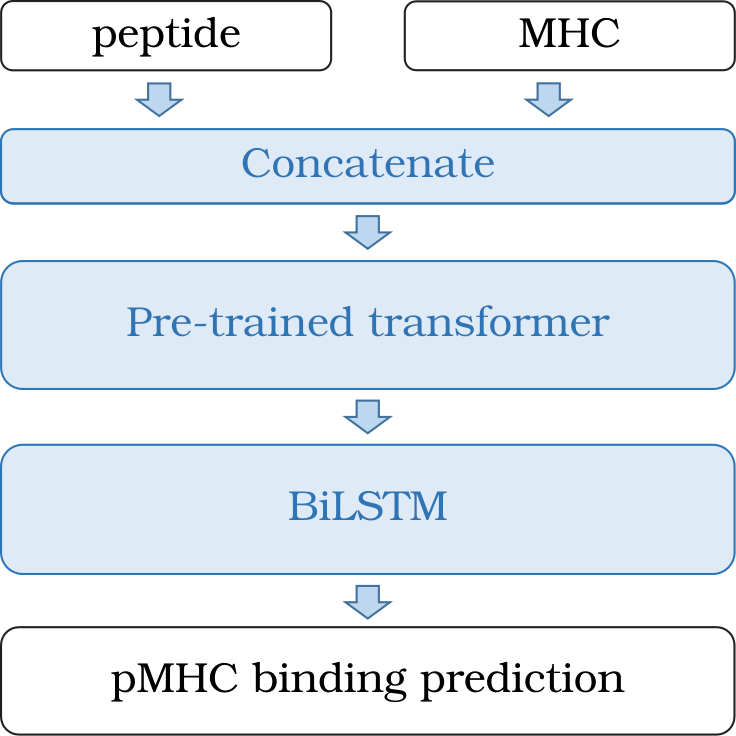
\includegraphics[width=0.7\textwidth]{img/neoantigen/fine_tune2}
		\caption{Transformer model.}
		\label{fig:finetune}
	\end{subfigure}
	\hfill
	\begin{subfigure}[b]{0.56\textwidth}
		\centering
		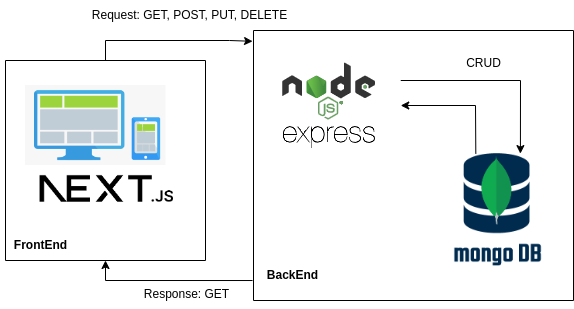
\includegraphics[width=\textwidth]{img/neoantigen/web_arch}
		\caption{Web platform architecture.}
		\label{fig:web}
	\end{subfigure}
	
	\caption{(a) The proposed model for PPI prediction of peptides and MHC. (b) The Web architecture.}
	\label{fig:proposal}
\end{figure}


Table \ref{tab:plan} presents the work plan for each three months. We consider 24 months for developing, training models, and deploying our proposal. 

\begin{table}[H]
	\centering
	\setlength{\tabcolsep}{0.5em} % for the horizontal padding
	{\renewcommand{\arraystretch}{1.2}% for the vertical padding
		\caption{Proposal work plan for each three months.}
		\label{tab:plan}
		\begin{tabular}{|p{7.4cm}|p{2.3cm}|c|c|c|c|c|c|c|c|} \hline
			\textbf{Activities}                                  &   \textbf{Outcome}         & I & II & III & IV & V & VI & VII & VIII \\ \hline
			
			\textbf{Milestone I} &  Models & & & & & & & &\\
			Literature review       &                       & x                     & x                      & x                       &                       &                       &                        &  &                                                \\
			Transformers model development  &                           &       x                &           x             &                x         &                       &                       &                        &              &                                  \\
			Training TAPE, ProtBert-BFD and ESM-2  &                           &                       &           x             &                x         & x                      &                       &                        &              &                                  \\
			Hyper-parameters tuning  &                           &                       &           x             &                x         & x                      &                       &                        &              &                                  \\
			Comparison with state-of-art methods &    &                       &                        & x                       & x                      & x                     &                        &            &                                       \\ \hline
			
			\textbf{Milestone II} & Web platform & & & & & & & & \\
			Requirements definition &  &     x                &    x                    &            x             &                       &                      &                       &                               &                   \\
			Design and development &  &                     &                        &                 x        & x                      & x                     & x                      &                               &                   \\
			Testing and quality assurance &  &                     &                        &                         & x                      & x                     & x                      &                               &                   \\
			Deployment  &                                      &                       &                        &                         &                        &                      &                       & x                                         & x    \\
			Paper redaction and submission    &                              &                       &                        &                         &              x         &             x         &                x       & x                                       & x     \\ \hline
		\end{tabular}
	}
\end{table}

\subsection{EMBL group and partnership organization}
I consider that the \textit{Bateman group} of EMBL led by Alex Bateman is the most suitable group to support this research. Because its future goals aim to use deep learning methods to embed protein sequences. In this context, my project proposes fine-tuning transformers trained on large protein databases for predicting pMHC bindings. After training, the model saved PPI representation in the model's last layers, so we could use it to get embeddings from pairs of protein sequences; it opens new ways to investigate proteins.


Furthermore, this research project will benefit from collaboration with 
\textit{Institut Curie}. This partner aligned perfectly with my research interests and my current project, because of its support in immunology, cancer translational research, and proteomics.

\subsection{Infrastructure}

The requirements area based on the resources for training the transformers and Web platform hosting. They are detailed in Table \ref{tab:infrastructure}.

\begin{table}[]
	\caption{List of infrastructure requirement.}
	\label{tab:infrastructure}
	\begin{tabular}{lll}
		\textbf{Infrastructure}                                    & \textbf{Cost}  & \textbf{Available at} \\ \midrule
		GPU like V-100 or A-100 to train transformer models        & 200\$          & HuggingFace           \\
		Hosting for Web platform with Mongo, Express.js and Python & 0.5\$ per hour & EMBL                 
	\end{tabular}
\end{table}


\subsection{Potential risks }

\begin{itemize}
	\item A lack of resources in order to train large transformer models. This is currently the most challenging problem for junior researchers; nevertheless, I faced this problem last year, and there are no expensive cloud services that I could use.
\item No available hosting services at EMBL. I consider that AWS credits could finance this risk at the beginning until EMBL hosting services are available.
\end{itemize}

\section{Expected results and their impact}
\subsection{When do you expect to be able to start providing (pilot) access?}
After the first year of the fellowship, I can grant access to some users. This pilot will include a simple Web page with functionalities for predicting PPI interactions on the first trained models. 

\subsection{Will the technology be useful to other EMBL groups?}
Yes, the \textit{Protein Function Development} group because PPI interaction plays a key role in protein function prediction. Additionally, one of its last publications \cite{dalkiran2023transfer} used deep learning and transfer learning for drug-target interaction prediction in a similar way to my proposal. Finally, with the use of first-hand protein data from UniProt FTP site (disseminated by this group), a huge transformer model could be trained to solve similar problems in PPI prediction and protein annotation.\\


\subsection{Which external (non-EMBL) researchers could be first users?}
All research groups that study immunology. For instance, \textit{the Parker Institute for Cancer Immunotherapy} and the \textit{Cancer Research Institute} are researching cancer neoantigens to develop personalized vaccines. They are potential users because neoantigen detection depends on several steps; however, one of the most relevant is the prediction of bindings between peptides to the MHC; if it occurs, these peptides are potential neoantigens.

\subsection{Service provision}
The main functionality is the prediction of pMHC bindings. The user must provide a list of peptides and the MHC sequence. Then, the Web platform will store this request in a job, and after finishing, an email will be delivered to the user with its results. Additionally, an API with the same functionality explained before will be available for research groups. \\

Approximately the time to deliver the user's results will depend on the amount of peptides included in the request and the current number of jobs waiting for processing. However, for a single request of 100 peptides, the server should take 3 minutes if the server has a GPU like RTX-3070 (I measure this time on similar projects).\\

Furthermore, the main obstacles related to service provision are future problems with the server workload and the limitation of the server's GPU specifications. 


\section{Ethics}
N/A.

\section{Gantt chart}

The activities and milestones are detailed in Table \ref{tab:plan} and Figure \ref{fig:gantt}.

\begin{figure}[h]
	\centering	
	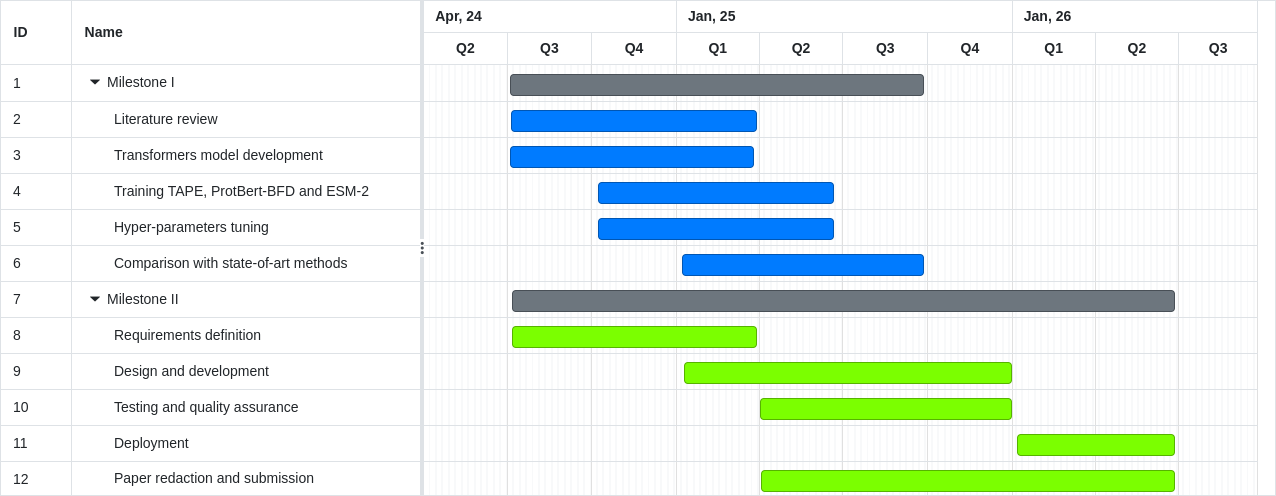
\includegraphics[width=\textwidth]{img/neoantigen/gantt}
	\caption{Gantt chart for the project proposal.}
	\label{fig:gantt}
	
\end{figure}
	
	


	
	%\bibliographystyle{apalike}
	\bibliographystyle{IEEEtran}
	\bibliography{bibliography}
	
\end{document}